\atstartofhistorysection
\section[Un peu d’histoire : l’aventurier Rumford]{Un peu d’histoire :\onlyamphibook{\\} Rumford, un aventurier qui «~pèse~» la chaleur}
\label{ch_histoire_rumford_depondt}

\begin{center}\textit{Par Philippe Depondt\\ \begin{small}Université Pierre et Marie Curie, Paris\\ Contribution sous licence \ccbysa\end{small}}\end{center}

	Il s'appelait en fait Benjamin Thompson (1753-1814) et était américain de Woburn, Massachussetts~\cite{millar1996}. Il eut d'abord de nombreuses et éclectiques occupations : employé dans un magasin, instituteur, étudiant en médecine…\ Toutefois, quand la révolution américaine survint, la Nouvelle Angleterre où il habitait se trouva au cœur du conflit ; Thompson choisit le camp loyaliste et devint agent secret pour les Anglais. Au moment de la déclaration d'indépendance des États-Unis d'Amérique en 1776, prudemment, il partit pour l'Angleterre.

	Il entreprit alors des recherches sur les projectiles et entra à la \textit{Royal Society} en 1779. Il retourna cependant en Amérique en 1782 toujours pour y combattre du côté anglais, mais la paix fut déclarée l'année suivante. Il fut anobli baron Rumford par le roi George \textsc{iii} en récompense de ses services. Il devint alors conseiller de l'électeur de Bavière, puis ministre de la guerre. Pendant les 14 ans passés en Bavière, il réforma l'armée, institua des aides pour les nécessiteux, créa le célèbre «~Jardin Anglais~»\ (\textit{Englisher Garten}) à Munich. Il retourna ensuite en Angleterre, pour finalement s'installer en France en 1805 où il fit un mariage --désastreux-- avec Marie Lavoisier, la veuve du chimiste décapité pendant la révolution française.

	Au cours de cette vie aventureuse, il trouva le moyen de faire au moins deux découvertes importantes. Dans le cadre de la théorie du calorique, il tenta de peser la chaleur, en pesant des corps portés à différentes températures. De ces tentatives infructueuses, il déduisit que la chaleur n'a pas de poids. Ensuite, au cours de ses activités de ministre de la guerre, il faisait forer des canons et observa en 1798 que l'action du forage échauffait les fûts au point de faire bouillir de l'eau. Il comprit que la quantité de chaleur ainsi dégagée n'était pas limitée par la quantité de matière qui la contenait. Il en déduisit que cette chaleur n'était pas contenue dans la matière mais \emph{produite} par le travail des chevaux qui actionnaient le foret : une préfiguration du premier principe de Joule.

	L'histoire des sciences comporte aussi quelques personnages plutôt romanesques !

	\begin{figure}
		\begin{center}
			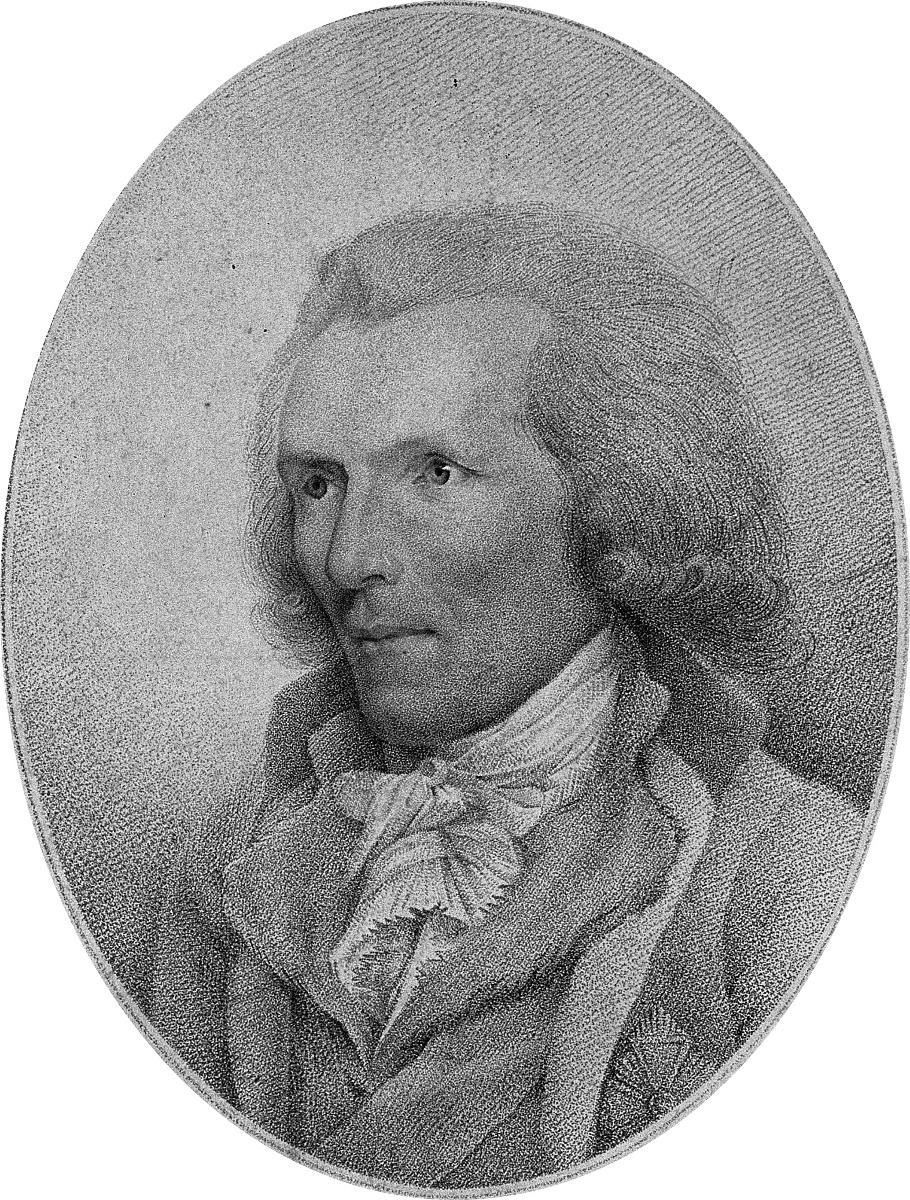
\includegraphics[width=5cm]{images/benjamin_thompson.jpg}
			\supercaption{Sir Benjamin Thompson de Rumford, combattant milicien, agent secret, architecte, ministre de guerre, expérimentateur hardi, séducteur cosmopolite, et bien sûr, thermodynamicien.}%
			{\wcfile{Sir Benjamin Thompson, Count von Rumford. Stipple engraving Wellcome V0005796.jpg}{gravure} par  J. P. P. Rauschmayr, 1797 (\pd)}
			\label{fig_benjamin_thompson}
		\end{center}
	\end{figure}


\atendofhistorysection
